\documentclass[10pt,a4paper]{beamer}

%\usepackage[applemac]{inputenc}
\usepackage[ngerman]{babel}
\usepackage[utf8]{inputenc}
\usepackage{times}
\usepackage{graphicx}
\usepackage{setspace} %Zeilenabstand?
\usepackage{wrapfig} %Benoetigt fuer Textumflossene Bilder
\usepackage{hyperref}
\usepackage{marvosym} %Symbol Link
\usepackage{fontawesome5}
%%%%%%%%%%%%%%%%%%%%%%%%%%%%%%%%%%%%%%%%%%%%%%%%%%%%%%%%%%%%%%%%%%%%%%%%%%%%%%%%
\usetheme{Boadilla}
\definecolor{ecs100}{RGB}{60, 119, 20}
\setbeamercolor{structure}{fg=ecs100,bg=white}

\setbeamertemplate{section in toc}[default]

\setbeamertemplate{itemize items}[circle]
\setbeamertemplate{enumerate items}[default]



\setbeamertemplate{headline}
{%
    \vspace*{2.5ex}%
    \begin{beamercolorbox}[wd=0.09\textwidth,ht=2ex,dp=0.5ex,leftskip=.5em,rightskip=.5em]{author in head/foot}%
        \usebeamerfont{author in head/foot}%
        Folie \insertframenumber%
    \end{beamercolorbox}%
    \vspace*{+0.02ex}%
    \hspace*{0.07\textwidth}%
    \begin{beamercolorbox}[wd=0.92\textwidth,ht=1.9ex,dp=0.5ex,right,leftskip=.5em]{title}%
        \begin{picture}(0,0)
            \put(0,0.5){\rule[1.8ex]{\textwidth}{0.2ex}}
        \end{picture}% 2ex - 0.2ex = 1.8ex
        {\usebeamerfont{title in head/foot}%
        \qquad \insertshorttitle \ \ $\vert$ \ \ \insertshortsubtitle \ \ $\vert$ \ \ \insertshortdate \hfill \insertsubsection $\leftarrow$\insertsection \break
        }
    \end{beamercolorbox}%
}

\setbeamertemplate{frametitle}
{%
    \vspace*{1ex}%
    \usebeamercolor{title} \bf \large \insertframetitle%
    \vspace*{-0.5ex} }

\setbeamertemplate{footline}{} % Fußzeile aktivieren/deaktivieren
\setbeamertemplate{navigation symbols}{} % Navigationsfunktion aktivieren/deaktivieren
%%%%%%%%%%%%%%%%%%%%%%%%%%%%%%%%%%%%%%%%%%%%%%%%%%%%%%%%%%%%%%%%%%%%%%%%%%%%%%%%%%%%%%%%%%%
%Die eigenen Daten hier einfügen:

\date[WS 2022/2023]{Ulm, WS 2022/2023}
\title[CSE]{Studienbeginn CSE - WS 22/23}
\subtitle[Studienbeginn]{\hspace{1cm} Fachschaft CSE}

\setcounter{framenumber}{-1}

%MY DEFINITIONS BEGIN
\def\r#1{{\color{red}#1}}
\def\g#1{{\color{green}#1}}
\def\mg#1{{\color{ecs100}#1}}
\def\titlefont#1{\textbf{\large\mg{#1}}}
%MY DEFINTIONS END

%BEGIN DOCUMENT
\begin{document}


%Titel Seite
    \frame[plain]{
        \vspace*{-0.3cm}
        \flushright 
\includegraphics[width=.2\textwidth]{logo_fs-cse.png}
%	\leftskip-2.58em%
        \vspace{-0.2cm}
        \begin{center}
            \makebox[\textwidth]{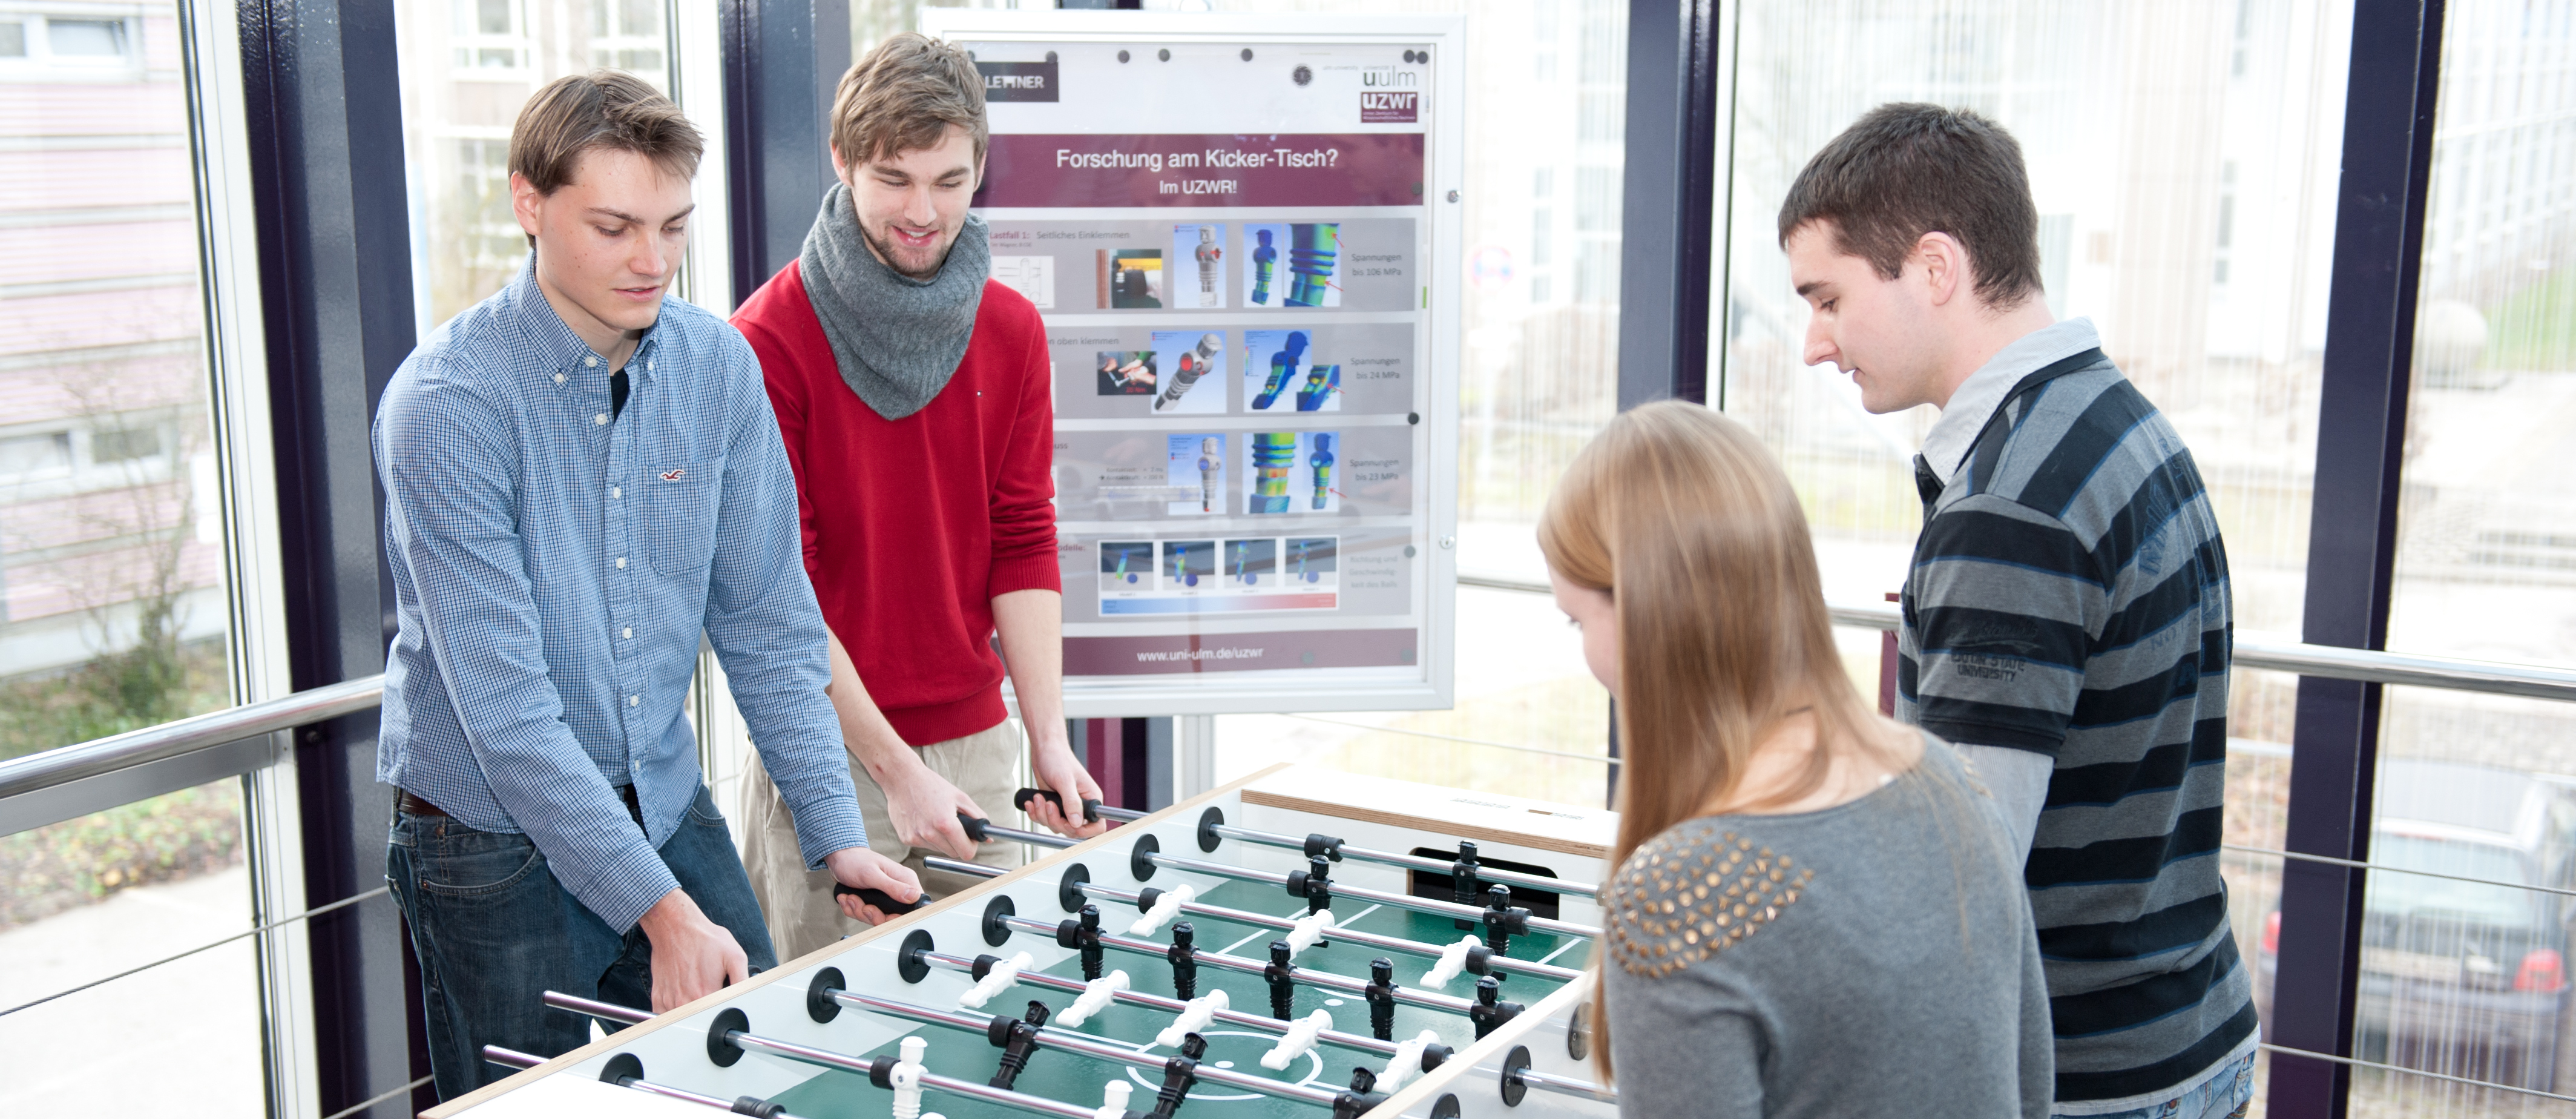
\includegraphics[width=\paperwidth]{tischkicker-wide.jpg}}
        \end{center}

    %\vspace*{1cm}
        \begin{center}
            \textcolor{ecs100}{\hspace{-5cm}\Large  \inserttitle}
        \end{center}
    }


% Das Inhaltsverzeichnis


%%%%%%%%%%%%%%%%%%%%%%%%%%%%%%%%%%%%%%%%%%%%%%%%%%%%%%%%%%%%%%%%%%%%%%%%%%%%%%%%%%%%%%%%%%%
%Ab hier beginnt die Präsentation:
% 1. Folie: Inhaltsverzeichnis
    \begin{frame}
        \frametitle{Inhaltsverzeichnis}
        \tableofcontents
        % [pausesections] % Animation/Einblendung der einzelnen Abschnitte
    \end{frame}

%%%%%%%%%%%%%%%%%%%%%%%%%%%%%%%%%%%%%%%%%%%%%%%%%%%%%%%%%%%%%%%%%%%%%%%%%%%%%%%%%%%%%%%%%%%
%Ab hier beginnt die Präsentation:


    \section{eduroam}
    \begin{frame}
        \frametitle{eduroam}
%\makebox[\textwidth]{\includegraphics[width=\paperwidth]{eduroam.png}}
        \begin{center}
            \includegraphics[width=0.5\paperwidth]{eduroam.png}
        \end{center}
%\includegraphics[width=0.5\paperwidth]{eduroam.png}
        \begin{itemize}
            \item https://www.uni-ulm.de/einrichtungen/kiz/service-katalog/netzwerk-konnektivitaet/wlan/eduroam/
        \end{itemize}
% https://www.uni-ulm.de/einrichtungen/kiz/service-katalog/netzwerk-konnektivitaet/vpn/
    \end{frame}


    \section{Grundsätzliches}
    \begin{frame}
        \frametitle{Grundsätzliches}
        \begin{center}
            
\includegraphics[width=0.7\paperwidth]{Logos.png}
        \end{center}
        \vspace{0.3cm}
        \begin{itemize}
            \item Kooperationsstudiengang der Universität und Technischen Hochschule Ulm
            \begin{itemize}
                \setlength{\itemsep}{10pt} %Zeilenabstand ändern
                \item Zwei Studierendenausweise
                \item Doppeltes Angebot beim Hochschulsport, Orchestern etc.
                \item Unterschiedlichen Regelungen
                \item Vorlesungen an verschiedensten Standorten
            \end{itemize}
        \end{itemize}
    \end{frame}

    \begin{frame}
        \begin{center}
            \makebox[\textwidth]{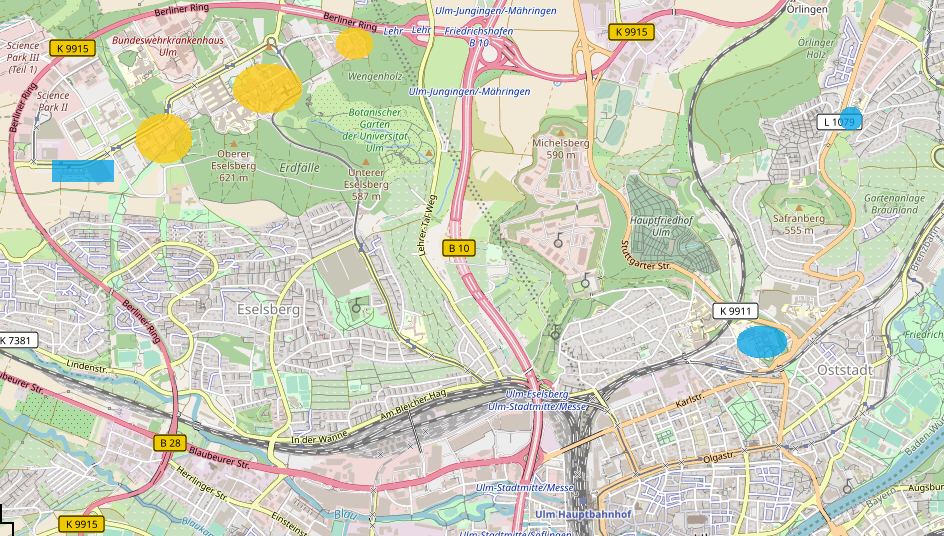
\includegraphics[width=\paperwidth]{Ulm.png}}
        \end{center}
    \end{frame}

    \begin{frame}
        \begin{center}
            \makebox[\textwidth]{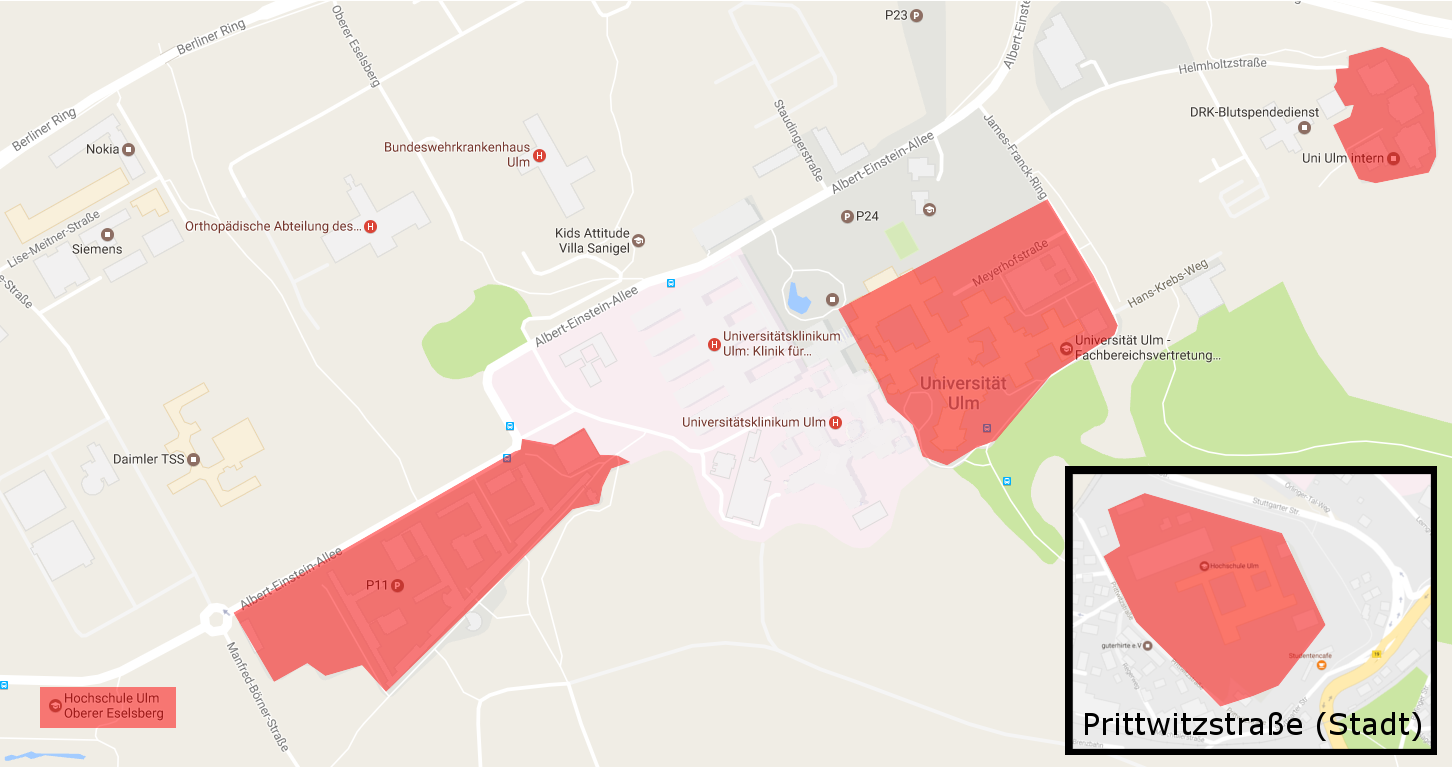
\includegraphics[width=\paperwidth]{karte.png}}
        \end{center}
    \end{frame}


    \section{Vorlesungszeiten}
    \begin{frame}
        \frametitle{Vorlesungszeiten}
        \begin{itemize}
            \setlength{\itemsep}{10pt} %Zeilenabstand ändern
            \item Semesterbeginn / -ende

            \begin{itemize}
                \setlength{\itemsep}{10pt} %Zeilenabstand ändern
                \item THU: 27.09.2022 - 20.01.2023 \\ (Vorlesungsfreie Zeit um Weihnachten: 24.12.2022 - 09.01.2023)
                \item Uni: 17.10.2022 - 18.02.2023\\(Vorlesungsfreie Zeit um Weihnachten: 24.12.2022 - 05.01.2023)
            \end{itemize}

            \item cum tempore / sine tempore:
            \begin{itemize}
                \setlength{\itemsep}{10pt} %Zeilenabstand ändern
                \item Uni: c.t., d.h. die Vorlesung beginnen \emph{Viertel nach}
                \item HS: s.t., d.h. die Vorlesungen beginnen \emph{um Punkt}
                \item Bei Prüfungen: Hinweise beachten
            \end{itemize}
        \end{itemize}
    \end{frame}


    \section{Studentenausweise}
    \begin{frame}
        \frametitle{Studentenausweise}
        \begin{itemize}
            \setlength{\itemsep}{10pt} %Zeilenabstand ändern
            \item Zwei Studentenausweise mit identischer Matrikelnummer
            \item Verschiedene Konten auf den einzelnen Ausweisen
            \item Verlängerung jedes Semester jeweils an einem Automaten der THU und einem SB-Terminal in der Uni (PIN wird benötigt!)
            \item Kostenlose Fahrt im DING-Netz ab 18h sowie am Wochenende und an Feiertagen
            \item Beim Kauf eines Semestertickets unterschiedliche Semesterzeiträume der THU und Universität beachten
        \end{itemize}
    \end{frame}

    \subsection*{Studentenausweis Universität}
    \begin{frame}
        \frametitle{Studentenausweis Universität}
        \begin{itemize}
            \setlength{\itemsep}{10pt} %Zeilenabstand ändern
            \item Zugangskarte zu PC-Pools sowie nachts zur Universität
            \item Bezahlmittel mit drei verschiedenen Konten:
            \begin{itemize}
                \setlength{\itemsep}{10pt} %Zeilenabstand ändern
                \item \textbf{Mensa} (Aufwertung durch Terminals oder am Info-Point) / \\ Bezahlen auch in den Mensen der THU möglich
                \item \textbf{Parken} (Aufwertung durch Automaten bei den Parkplätzen)
                \item \textbf{Druckkontingent} (Umbuchung am SB-Terminal, 16 Euro pro Kalenderjahr frei)
                \item \textbf{Druck- und Kopierkonto} (für Drucker von Ricoh, zusätzlich)
            \end{itemize}
            \item Identifikationsmittel bei Prüfungen
        \end{itemize}
    \end{frame}

    \subsection*{Studentenausweis Technische Hochschule}
    \begin{frame}
        \frametitle{Studentenausweis Technische Hochschule}
        \begin{itemize}
            \setlength{\itemsep}{10pt} %Zeilenabstand ändern
            \item Bezahlmittel an den Mensen der Technische Hochschule oder Universität
            \item Identifikationsmittel beim Drucken % (10 Euro pro Semester frei)
            \item Zugang zu den \textbf{kostenlosen} Parkplätzen der Technische Hochschule
            \item Identifikation bei Prüfungen
        \end{itemize}
    \end{frame}

% \section{Modulwahl}
% \begin{frame}
% \frametitle{Modulwahl}
% \begin{itemize}
% 	\setlength{\itemsep}{10pt} %Zeilenabstand ändern
% 	\item \href{https://www.uni-ulm.de/mawi/mawi-cse/studierende/master-cse/wahlpflicht-ma-cse/}{\Mundus~Allgemeine Informationen}
% 	\item \href{https://goo.gl/R8cisD}{\Mundus~Modulhandbuch Uni}
% 	\item \href{https://goo.gl/Ad3BQm}{\Mundus~Modulhandbuch HS}
% \end{itemize}
% \end{frame}


    \section{Accounts und Portale}
    \begin{frame}
        \frametitle{Accounts und Portale}
        \begin{itemize}
            \setlength{\itemsep}{10pt} %Zeilenabstand ändern
            \item E-Mails
            \begin{itemize}
                \setlength{\itemsep}{10pt} %Zeilenabstand ändern
                \item https://sogo.uni-ulm.de/SOGo/
                \item https://webmail.hs-ulm.de
            \end{itemize}
            \item LSF
            \begin{itemize}
                \setlength{\itemsep}{10pt} %Zeilenabstand ändern
                \item \textbf{https://campusonline.uni-ulm.de}
                \item https://lsf.verwaltung.hs-ulm.de
            \end{itemize}
            \item Moodle
            \begin{itemize}
                \setlength{\itemsep}{10pt} %Zeilenabstand ändern
                \item https://moodle.uni-ulm.de
                \item https://moodle-thu.de
            \end{itemize}
        \end{itemize}
    \end{frame}


    \section{Prüfungsanmeldung}
    \begin{frame}
        \frametitle{Prüfungsanmeldung}
        \begin{itemize}
            \setlength{\itemsep}{10pt} %Zeilenabstand ändern
            \item Anmeldung spätestens \textbf{vier Tage vor der Prüfung}, danach ist auch ein Rücktritt von der Anmeldung nicht mehr möglich
            \item Alle Prüfungen müssen über das Portal der Uni Ulm angemeldet werden, \textbf{nicht} über die Hochschule
            \item bei Fragen an die \href{https://www.uni-ulm.de/mawi/mawi-cse/studienfachberatung/}{\Mundus~Studienfachberatung CSE} wenden
            \begin{itemize}
                \setlength{\itemsep}{10pt} %Zeilenabstand ändern
                \item Beate Mayer (Universität Ulm) - beate.mayer@uni-ulm.de
                \item Kirsten Huss (Hochschule Ulm) - huss@hs-ulm.de
            \end{itemize}
        \end{itemize}
        \begin{alertblock}{Sonderregelung der Universität im WS}
            Die Anmeldung muss weiterhin spätestens vier Tage vor der Prüfung geschehen, aber dann ist noch bis ein Tag vor der Prüfung ein Abmeldung möglich!
        \end{alertblock}
    \end{frame}


    \section{Fachschaft CSE}
    \begin{frame}
        \frametitle{Fachschaft CSE}
        \begin{itemize}
            \setlength{\itemsep}{10pt} %Zeilenabstand ändern
            \item FS CSE ist nicht eigenständig, sondern ein Teil der FS Mathe
            \item Treffen: Alle zwei Wochen im Vorlesungszeitraum, genaue Informationen auf unserer Website.
            \item Cloud mit Altklausuren / Material aus älteren Semestern
            \item Erreichbar über:
            \begin{itemize}
                \item \href{https://www.facebook.com/groups/356850697732243/}{\Mundus~Facebook}
                \item \href{https://chat.whatsapp.com/CQYUbnH2UGZLXuFFrI0VxO}{\Mundus~WhatsApp}
                \item E-Mail: fs-cse@uni-ulm.de
            \end{itemize}
        \end{itemize}
    \end{frame}

    \begin{frame}
        \frametitle{ \href{http://fs-cse.de}{\Mundus~fs-cse.de}}
        \begin{center}
            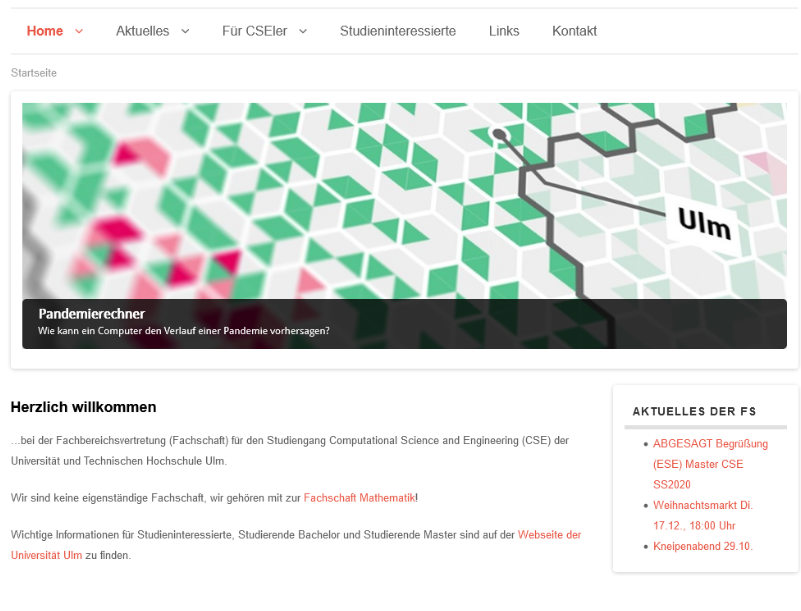
\includegraphics[width=0.85\textwidth]{website.png}
        \end{center}
    \end{frame}
    \begin{frame}
        \frametitle{\href{http://cloud.fs-cse.de}{\Mundus~cloud.fs-cse.de} }
        \begin{itemize}
            \setlength{\itemsep}{10pt} %Zeilenabstand ändern
            \item Sammlung von Skripten, Übungsaufgaben, Altklausuren
            \item Registrierung über \href{http://cloud.fs-cse.de/register/}{\Mundus~cloud.fs-cse.de/register/} (\textbf{nur} im Uninetz, oder via VPN/webVPN)
            \item Jeder kann in den Ordner \emph{Datenaustausch} Dateien hochladen
            \item Diese Präsentation liegt im Ordner CSE-Bachelor
        \end{itemize}
    \end{frame}

    \begin{frame}
        \frametitle{UniNow}
        \begin{center}
            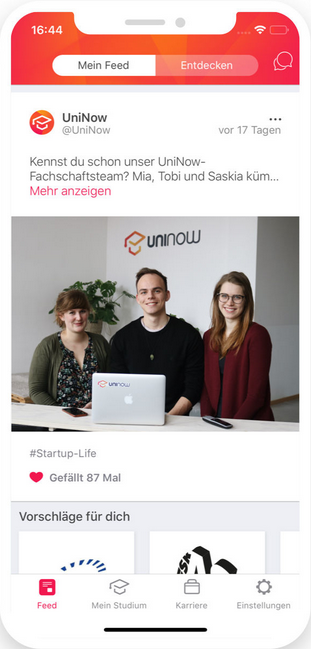
\includegraphics[height=0.7\textheight]{uninow1.png}
            \hspace{1cm}
            
\includegraphics[height=0.7\textheight]{uninow2.png}
        \end{center}
        \begin{block}{Folge uns auf UniNow}
            https://uninow.page.link/FS-CSE
        \end{block}
    \end{frame}

    \begin{frame}
        \frametitle{Weitere Tipps \& Tools}
        \vfill
        \textbf{Tipps:}
        \vfill
        \begin{itemize}
            \item Netzwerk aufbauen – sowohl mit Kommilitonen als auch mit Professoren.
            \vfill
            \item Lernen lernen – wie lernst du?
            \vfill
            \item Bafög - bequemes \href{https://www.bafoeg-digital.de/}{\color{ecs100}Online-Portal}, alles digital (nutzt die E-Ausweisfunktion!). Mehr Infos \href{https://studierendenwerk-ulm.de/bafoeg-finanzen/}{\color{ecs100}hier}.
        \end{itemize}
        \vfill
    \end{frame}

    \begin{frame}
        \frametitle{Weitere Tipps \& Tools}
        \vfill
        \textbf{Tools:}
        \vfill
        \begin{itemize}
            \item \textbf{Anki\,
\includegraphics[height=10pt]{bilder/anki.png}:} Eine nützliche App für Karteikarten.
            \vfill
            \item \textbf{GitHub\,\faIcon{github} (/git):} Eine Cloud-Plattform für deinen Code.
            \vfill
            \item \textbf{Overleaf\,
\includegraphics[height=10pt]{bilder/overleaf.png}:} Eine Online-Plattform für kollaboratives Schreiben und Teilen von LaTeX-Dokumenten.
            \vfill
            \item \textbf{VS Code\,
\includegraphics[height=10pt]{bilder/vs-code.png}:} Ein leistungsstarker Code-Editor mit vielen Erweiterungen für verschiedene Programmiersprachen.
            \vfill
            \item \textbf{Notabilitiy\,
\includegraphics[height=10pt]{bilder/notability.png}:} Eine App zur digitalen Notizen- und Handschriftenerfassung (iPad).
            \vfill
            \item \textbf{Notion\,
\includegraphics[height=10pt]{bilder/notion.png}:} Eine vielseitige Plattform für Notizen und Organisation.
            \vfill
            \item \textbf{Reclaim\,
\includegraphics[height=10pt]{bilder/reclaim.png}:} Eine KI App für automatisierte Terminplanung, die dir bei der effizienten Organisation deines Zeitplans helfen kann.
            \vfill
            \item \textbf{LinkedIn\,\faIcon{linkedin}:} Ein soziales Netzwerk zur beruflichen Vernetzung und Karriereentwicklung. Welche Jobs, Praktika, Auslandsaufenthalte machen oder haben andere (ehemalige) CSE-Studenten gemacht?
        \end{itemize}
        \vfill
    \end{frame}

    \begin{frame}
        \begin{center}
            \Huge{Noch Fragen?}
        \end{center}
    \end{frame}

\end{document}
